\documentclass[12pt]{article}
\usepackage[top=1in, bottom=1in, left=1in, right=1in]{geometry}
\usepackage[justification=centering]{caption}
\usepackage{graphicx}
\usepackage{listings}
\usepackage{color}
\usepackage{indentfirst}
\usepackage{hyperref}
\usepackage{siunitx}
\usepackage{float}

\lstset{ %
	%language=C,                % choose the language of the code
	basicstyle=\scriptsize,       % the size of the fonts that are used for the code
	                  % how far the line-numbers are from the code
	backgroundcolor=\color{white},  % choose the background color. You must add \usepackage{color}
	showspaces=false,               % show spaces adding particular underscores
	showstringspaces=false,         % underline spaces within strings
	showtabs=false,                 % show tabs within strings adding particular underscores
	%frame=single,           % adds a frame around the code
	tabsize=2,          % sets default tabsize to 2 spaces
	captionpos=b,           % sets the caption-position to bottom
	breaklines=true,        % sets automatic line breaking
	breakatwhitespace=false,    % sets if automatic breaks should only happen at whitespace
	escapeinside={\%*}{*)}          % if you want to add a comment within your code
}

\newcommand{\uz}{UART0}
\newcommand{\uo}{UART1}

\begin{document}
\title{Microprocessor Systems\\ Lab 3: Asynchronous \&\ Synchronous Serial Communications }
\author{Nick Choi \and Samuel Deslandes}
\date{10/17/16}
\maketitle
\pagebreak
\section{Introduction}


\section{Methods}
\subsection{Software}
The code for parts 1, 2 and 3 can be found in the appendix below. All code was uploaded and run on the 8051 through the programming/debugging USB port. 	

\subsubsection{Part 1}
The purpose of C program for the first section of the lab was to write a procedure that would monitor the UART0 and UART1 serial ports continuously, and echo a message received on one port to the other. For this section of the lab, this was accomplished by polling the receive interrupt flags RI0 and RI1 for UART0 and UART1 respectively. 

Since this lab uses both UART0 and UART1, both ports must be enabled on the crossbar. The enable bit for UART0 can be found on the XBR0 SFR, XBR2 for that of UART1. As always, the crossbar enable bit in XBR2 must be set. UART0 was configured to be in mode 1 (8-bit UART with variable baud rate), and use Timer2 to generate a baud rate of \si{9600}{bps}. UART0 configuration can set in the SSTA0 and SCON0 SFRs. Timer2 was configured to be in auto-reload mode and use SYSCLK as a base. These settings can be found in the TMR2CN and TMR2CF SRFs. To count to 9600, the reload value must be set to \texttt{0xFEBC}. This was calculated as follows:\\
\begin{equation}
	\mathtt{Mode1\_BaudRate} = \frac{\mathtt{SYSCLK}}{16*(65536-\mathtt{ReloadValue})}
\end{equation}\\
For a desired baud rate of 9600 and SYSCLK of \si{49,766,400}{Hz}, this comes out to:\\
\begin{equation}
9600= \frac{49766400}{16*(65536-\mathtt{ReloadValue})}
\end{equation}
\begin{equation}
\mathtt{ReloadValue} = 65212
\end{equation}
This is equivalent to \texttt{0xFEBC} in hex.

UART1 was similarly configured, but used Timer1 to generate a baud rate of \si{115200}{bps}. UART1 can be configured in the SCON1 SFR. Timer1 was set to be an 8-bit counter with auto-reload, and use SYSCLK as a base; these changes can be made in the TMOD SFR. The Timer1 reload value should be set as \texttt{0xE5}. This was calculated as shown below:\\ 
\begin{equation}
\mathtt{Mode1\_BaudRate} = \frac{\mathtt{SYSCLK}}{16*(256-\mathtt{ReloadValue})}
\end{equation}
\begin{equation}
\mathtt{ReloadValue} = 229
\end{equation}\\
This is equivalent to \texttt{0xE5} in hex.

When configuring both UARTs be sure that the receive enable bits are set in the SCON SFRs and that the timers are have been started. In addition to this, in the P0MDOUT SFR configure the TX pins (P0.0, P0.2) as push-pull for outputs, and the RX pins (P0.1, P0.3) as open-drain for inputs; Also, in the P0 SFR set the inputs (RX pins) for high impedance. 

The main routine of this program consists of two sub-routines `checkSBUF()' and `echo()' which are run in an infinite loop. The `checkSBUF()' function continuously polls RI0 and RI1, and returns the value stored in the UART data register when one of the flags is set. The UART data register (SBUFn) is used for both a receive and a transmit buffer. When data is read from SBUF, as is the case for the `checkSBUF()' function, it comes from the receive buffer. When data is written to SBUF it goes to the transmit buffer and is eventually transmitted when a full byte has been written. The returned value from `checkSBUF()' is then passed into the `echo()' function, where it is loaded into both SBUF0 and SBUF1 for transmission to both terminals. Recall that SBUF0 and SBUF1 are on different pages, and that SFRPAGE should be changed accordingly. 

\subsubsection{Part 2}
This section of the lab was divided into two parts.
The task for the first part was similar to that of section 1, however rather than polling, interrupts were used. The second part involved connecting UART1 to that of another 8051, so that when data is sent to UART0 of one of the 8051s, it echoed to the UART0 of the other microcontroller. The initial configurations were all the same as they were in section 1, with the addition of having to set the global interrupt enable bit (EA), as well as the individual UART0 and UART1 interrupt enable bits which can be found on the IE and EIE2 SFRs respectively. With these bits set, whenever the transmit interrupt flags (TIn) or receive interrupt flags (RIn) are set, the CPU vectors to the appropriate interrupt service routine (ISR); These flags must be cleared manually by the software. The UART0 interrupt has a priority level of 4, while the \uo\ interrupt has a priority of 20. One thing to keep in mind in regard to these interrupts is that while UART0 interrupts are enabled, unless the UART0 and UART1 interrupt priorities are swapped, UART1 will not receive any interrupts. Since both receiving and transmitting will trigger an interrupt, the ISR must poll each flag to verify the source of the interrupt. 

For part 1 of this section of the lab, the main would only check if the command to end the program had been sent; everything else was handled in the ISRs. The \uz\ ISR checks if the source of the interrupt was a receive by checking if RI0 has been set. If so, it is cleared and the `echo()' subroutine is called. After this, \uz\ interrupts are temporarily disabled to allow \uo\ interrupts to go though. The \uo\ ISR has the same routine, however rather than disabling \uz\ interrupts, it re-enables them.

The program for part 2 was handled slightly differently. The main routine now continuously polled two flags `UART0\_flag' and `UART1\_flag', which would be set in the ISRs of UART0 and UART1 respectively. The `echo()' function is also used for this part, of the lab, but with the slight modification of disabling \uz\ interrupts before loading data into the SBUF registers. The \uz\ ISR checks whether the source of the interrupt is a receive, and if it is it clears RI0, reads SBUF0 into a global variable, and sets the \uz\_flag. The \uo\ ISR does the same, but enables \uz\ interrupts at the end of the ISR. 

In the main routine, once the \uz\_flag has been set, the program calls the `echo()' function, and clears the flag. If the \uo\_flag has been set, the program disables \uz\ interrupts, transmits the character to \uz\ via the SBUF0 register, re-enables \uz\ interrupts, then clears the flag. In this case, the character is sent only to \uz\ rather than being echoed to both ports to avoid a feedback loop of infinite transmissions between the two microcontrollers.

In order to allow interrupts on \uo\ to go through, in the main routine there is a brief period of time in which \uz\ is disable. This small window was implemented by incrementing a variable to 255 in a for loop.


\subsubsection{Part 3}
The third section of this lab deals with the serial peripheral interface bus (SPI), a synchronous serial communication interface. The goal of this section was to communicate with the 68HC11 as a slave device, and use it to echo back any characters that get sent to it. Although the primary focus of this lab is SPI, UART0 is also used to send data to the terminal. As was the case with UART, SPI must also be enabled on the crossbar to function. It's enable bit can be found on XBR0. The relevant configuration SFRs for SPI are SPI0CFG, SPI0CN, and SPI0CKR. In SPI0CFG, enable master mode, so that the 8051 acts as the master device. In the SPI0CN register, enable SPI0, and set it to operate in 4-wire single master mode. The SPI0CKR register stores data pertaining to SPI clock rate, which can be calculated as follows:\\
\begin{equation}
SCK = \frac{SYSCLK}{2\times(SPI0CKR+1)}
\end{equation}\\
Setting SPI0CKR to \texttt{0x18} with a SYSCLK of 49,766,400 results in a SCK of \si{995,328}{Hz}. For SPI communication, in the P0MDOUT SFR, the SCK, MOSI, and NSS pins (P0.2, P0.4, P0.5 respectively) must be set to push-pull.

The program for this section used 3 sub-routines: `SPI0\_READ()', which handles receiving data from the slave device and outputting it to the terminal, `SPI0\_WRITE()', which handles receiving user input, and sending that data to a slave device, and `write\_dummy()' which sends a byte of garbage data (a dummy) to the slave device. The main routine simply waits for user input by polling RI0, and when set, clears the flag and calls the  `SPI0\_WRITE()' and `SPI0\_READ()' functions.

The `write\_dummy()' function first selects the slave by clearing NSSMD0. It then checks to make sure that SPI is not busy, then clears SPIF and writes a byte of data (\texttt{0xFE} in this case) to the SPI data register SPI0DAT. Like the UART data register SBUF, SPI0DAT is used both to receive and transmit. Checking that the SPI is not busy with a transmission can be done by monitoring bit 7 of the SPI0CFG register. SPIF is the SPI interrupt flag, which is set at the end of a data transfer. Like RIn and TIn, this flag must be cleared manually. 

The `SPI0\_WRITE()' function starts by loading the data in SBUF0 into a variable. It then selects the slave, ensures that SPI is not busy, clears SPIF, and loads the from the variable into SPI0DAT to be sent to the slave. It then waits for the transmission to end and clears SPIF. Because the slave device contains a second shift register, the echoed response will be delayed by one transmission. This is why dummy bytes must be read and written in between every actual read and write. The next step in the `SPI0\_WRITE()' routine is to read the dummy byte, which is done by selecting the salve and moving the dummy byte out of SPI0DAT. This program will output the dummy char to the terminal. After reading the dummy char, the input character (received on UART0) is displayed on the terminal and the `write\_dummy()' function is called. The `SPI0\_READ()' function follows the same procedure as reading the dummy byte.

The display is formatted using ANSI escape sequences to split the screen horizontally, with the top half used to display the input received on UART0, and the bottom half for the echoed character (received on the MISO pin of SPI). In order to make the two halves scroll independently, the scroll area must be redefined to the half being printed to before each print. A for loop was used to move the cursor down the appropriate amount of rows. This was all done using ANSI escape sequences.
\subsection{Hardware}
The hardware for section 1 involved connecting a DB9 adapter to be used at the UART1 port. A schematic for this can be viewed in the appendix below. The TD pin on the DB9 was connected to the input of a hex inverter, with the output connected to the RX1 pin of UART1 (P0.3). The TX1 pin (P0.2) was connected to the input of an inverter, with the output connected to the RD pin on the DB9. In order to establish a common ground between the adapter and the microcontroller, the ground pin on the DB9 was connected to pin 1 on the 60 pin bus (DGND), which was connected to the ground on the power supply used. 
 
Section 2 called for connecting the UART1s of two microcontrollers. This was done by connecting the TX1 pin of one 8051 to the RX1 pin of the other, and vice versa for the RX1 pin. A diagram of this can also be found in the appendix below.


\section{Results}




\section{Conclusion}





\pagebreak
\section{Appendices}
\subsection{Modified putget.h}
	\lstinputlisting{putget.h}
\subsection{Circuit Schematic for sections 1 and 3}
	\begin{figure}[H]
		\centering
		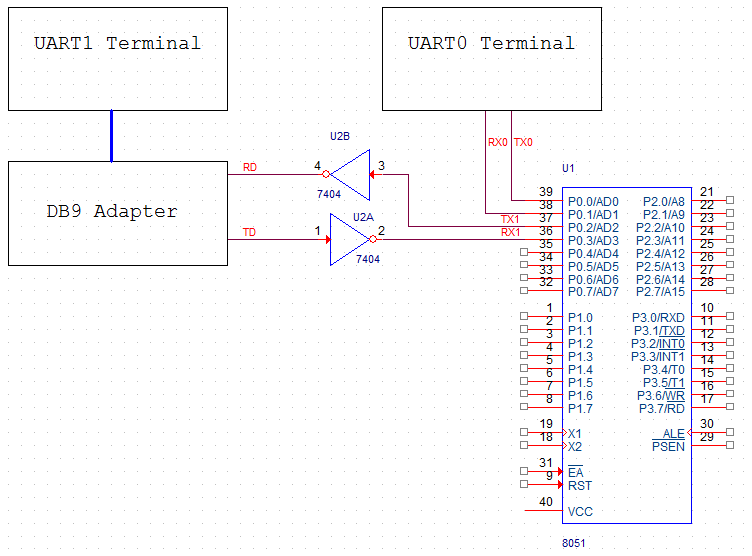
\includegraphics{Part1Schematic.png}
		\caption{Circuit schematic for parts 1 and 3}
		\label{schematic}
	\end{figure} 
\subsection{Part 1}
	\subsubsection{Code}
		\lstinputlisting{part1.c}
\subsection{Part 2}
	\subsubsection{Code}
		\lstinputlisting{part2-2v2_publish.c}	

%\pagebreak
\subsection{Part 3}
	%\pagebreak
	\subsubsection{Code}
		\lstinputlisting{part3-2_publish.c}
	
\section{References} 
\noindent
``MPS Lab 2," in RPI ECSE Department, 2016. [Online]. Available: \url{http://www.rpi.edu/dept/ecse/mps/MPS_Lab_Ex2-Intrpt.pdf}. Accessed: Sep. 22, 2016.\\
\newline\noindent
``C8051 Manual," in RPI ECSE Department, 1.4 ed., 2005. [Online]. Available: \url{https://www.ecse.rpi.edu/courses/CStudio/Silabs/C8051F12x-13x.pdf}. Accessed: Sep. 22, 2016.








\end{document}